%!TEX ROOT = main.tex

\section{Lab 1}

\subsection{Solution}

Lab 1 concerned the combinatorial optimisation of the set cover problem, which is NP-hard. The problem is to find a minimum set of subsets of a given set of subsets such that all elements of the given set are covered. Since a solution cannot be found in polynomail time, any implemented solution is guaranteed to be suboptimal. For this lab, the problem is tackled through a collection of search algorithms:

\begin{enumerate}
  \item Naive Greedy
  \item Greedy with a better cost function
  \item A* Traversal Using a Priority Queue
  \item A* Traversal Using a Fully Connected Graph
\end{enumerate}

\subsubsection{Naive Greedy}

\begin{mintedbox}{python}
  def naive_greedy(N):
    goal = set(range(N))
    covered = set()
    solution = list()
    all_lists = sorted(problem(N, seed=42), key=lambda l: len(l))
    while goal != covered:
        x = all_lists.pop(0)
        if not set(x) < covered:
            solution.append(x)
            covered |= set(x)

    print(
        f"Naive greedy solution for N={N}: w={sum(len(_) for _ in solution)} (bloat={(sum(len(_) for _ in solution)-N)/N*100:.0f}%)"
    )
\end{mintedbox}

The greedy algorithm essentially traverses through a sorted list of subsets and keeps adding the subset to the solution set if it covers any new elements. The algorithm is very naive as it does not take into account the number of new elements.

\subsubsection{Greedy with basic heuristic approximation}

This version of the greedy algorithm takes the subset with the lowest heuristic $f$ where $S_e$ is the expected solution (containing all the unique elements) and $n_i$ is the current subset:

\begin{equation*}
  f_i = 1 / |n_i - S_e|
\end{equation*}

In real-life scenarios, the cost depends on the relative price of visiting a node/choosing an option. Since we consider all options to be arbitrarily priced, we use a constant cost of 1.

\begin{mintedbox}{python}

def set_covering_problem_greedy(N, subsets, costs):
  cost = 0
  visited_nodes = 0
  already_discovered = set()
  final_solution = []
  expected_solution = set(list(itertools.chain(*subsets)))
  covered = set()
  while covered != expected_solution:
      subset = min(subsets, key=lambda s: costs[subsets.index(s)] / (len(set(s)-covered) + 1))
      final_solution.append(subset)
      cost += costs[subsets.index(subset)]
      visited_nodes = visited_nodes+1
      covered |= set(subset)
  print("NUMBER OF VISITED NODES: ", visited_nodes)
  print("w: ", sum(len(_) for _ in final_solution))
  print(
      f"Naive greedy solution for N={N}: w={sum(len(_) for _ in final_solution)} (bloat={(sum(len(_) for _ in final_solution)-N)/N*100:.0f}%)"
  )
  print(
      f"My solution for N={N}: w={sum(len(_) for _ in final_solution)} (bloat={(sum(len(_) for _ in final_solution)-N)/N*100:.0f}%)"
  )
  return final_solution, cost

  for n in [5, 10, 50, 100, 500, 1000]:
    subsets = problem(n, seed=SEED)
    set_covering_problem_greedy(n, subsets, [1]*len(subsets))
\end{mintedbox}

\subsubsection{A* Search Using a Priority Queue}

The A* algorithm requires a monotonic heuristic function that symbolises the remaining distance between the current state and the goal state. In the case of the set cover problem, the heuristic function is the number of elements that are not covered by the current solution set, such that finding all unique elements symbolises reaching the goal state. The algorithm is implemented using a priority queue.

The implemented algorithm can be surmised as pseudocode below:

\begin{enumerate}
  \item Add the start node to the priority queue
  \item While the state is not None, cycle through the subsets and compute the cost of adding this subset to the final list.
  \item If the cost has not been stored yet and the the new state is not in the queue, update the parent of each state. If travelling in this route produces a cheaper cost, update the cost of the node and its parent.
  \item Finally, compute the path we travelled through.
\end{enumerate}


\begin{mintedbox}{python}
  from typing import Callable
  from helpers import State, PriorityQueue
  import numpy as np

  class AStarSearch:
      def __init__(self, N, seed=42):
          # N is the number of elements to expect
          self.N = N
          self.seed = seed

      def add_to_state(self, st, subset):
          '''
          Unnecessary function to add a subset to a state because we are using the State class instead of a normal np.array
          '''
          state_list = st.copy_data().tolist()
          state_list.append(subset)
          return State(np.asarray(state_list, dtype=object))

      def are_we_done(self, state):
          '''
          Check if we have reached the goal state (such that all elements are covered in range(N))
          '''
          flattened_list = self.flatten_list(state.copy_data().tolist())
          for i in range(self.N):
              if i not in flattened_list:
                  return False
          # print("We are done")
          return True

      def flatten_list(self, l):
          '''
          Utility function to flatten a list of lists using itertools
          '''
          return list(itertools.chain.from_iterable(l))

      def h(self, state):
          '''
          Heuristic Function h(n) = number of undiscovered elements
          '''
          num_undiscovered_elements = len(set(range(self.N)) - set(self.flatten_list(state.copy_data().tolist())))
          return num_undiscovered_elements

      def astar_search(
          self,
          initial_state: State,
          subsets: list,
          parents: dict,
          cost_of_each_state: dict,
          priority_function: Callable,
          unit_cost: Callable,
      ):
          frontier = PriorityQueue()
          parents.clear()
          cost_of_each_state.clear()

          visited_nodes = 1
          state = initial_state
          parents[state] = None
          cost_of_each_state[state] = 0
          # to find length at the end without needed to flatten the state
          discovered_elements = []

          while state is not None and not self.are_we_done(state):
              for subset in subsets:
                  # if this list has already been collected, skip
                  if subset in state.copy_data():
                      # print("Already in")
                      continue
                  new_state = self.add_to_state(state, subset)
                  state_cost = unit_cost(subset)
                  # if new_state not in cost_of_each_state or cost_of_each_state[new_state] > cost_of_each_state[state] + state_cost:
                  if new_state not in cost_of_each_state and new_state not in frontier:
                      parents[new_state] = state
                      cost_of_each_state[new_state] = cost_of_each_state[state] + state_cost
                      frontier.push(new_state, p=priority_function(new_state))
                  elif new_state in frontier and cost_of_each_state[new_state] > cost_of_each_state[state] + state_cost:
                      parents[new_state] = state
                      cost_of_each_state[new_state] = cost_of_each_state[state] + state_cost
              if frontier:
                  state = frontier.pop()
                  visited_nodes += 1
              else:
                  state = None

          path = list()
          s = state

          while s:
              path.append(s.copy_data())
              s = parents[s]

          print(f"Length of final list: {len(self.flatten_list(path[0]))}")
          print(f"Found a solution in {len(path):,} steps; visited {len(cost_of_each_state):,} states")
          print(f"Visited {visited_nodes} nodes")
          print(
              f"My solution for N={self.N}: w={sum(len(_) for _ in path[0])} (bloat={(sum(len(_) for _ in path[0])-self.N)/self.N*100:.0f}%)"
          )
          return list(reversed(path))

      def search(self, constant_cost=False):
          GOAL = State(np.array(range(self.N)))
          subsets = problem(self.N, seed=self.seed)
          initial_state = State(np.array([subsets[0]]))

          parents = dict()
          cost_of_each_state = dict()

          self.astar_search(
              initial_state = initial_state,
              subsets = subsets,
              parents = parents,
              cost_of_each_state = cost_of_each_state,
              priority_function = lambda state: cost_of_each_state[state] + self.h(state),
              unit_cost = lambda subset: 1 if constant_cost else len(subset)
          )
\end{mintedbox}

The unit cost during search can either be set to a constant of 1 or the length of chosen subsets. The latter is employed as it helps the algorithm focus on finding all the elements with minimal overhead (redundant elements).

\subsubsection{A* Search with Fully Connected Graph (Failed Idea)}

An initial idea I had was to build a fully connected graph where each subset is in it's own node, and run an A* star search to traverse it and find a shortest path. For several logical and overhead reasons, this idea produced poor results and large bloats for big $N$s.

Given A = $[2, 4, 5]$, B = $[2, 3, 1]$ and C = $[1, 2]$,

\begin{figure}[h]
\centering
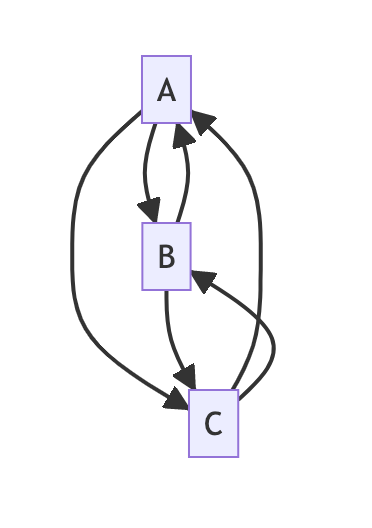
\includegraphics[width=0.3\textwidth]{images/astar.png}
\caption{Fully connected graph}
\label{fig:fully_connected_graph}
\end{figure}

The heuristic function is slightly different:

\begin{equation*}
h_i = len(s_i) - len(s_i \cap S_e)
\end{equation*}

where $s_i$ is the current subset and $S_e$ is the expected solution. It takes into account both the length of the new subset (to minimise final weight) and the number of undiscovered elements that it can contribute.

We can also immediately return a very large heuristic value such as 100 in the case of duplicating elements in the subset or in any situation where we want a certain node to be immediately skipped.

\begin{mintedbox}{python}
  class AStarSearchFullyConnectedGraph:
    def __init__(self, adjacency_list, list_values, N):
        self.adjacency_list = adjacency_list
        self.list_values = list_values
        H = {}
        for key in list_values:
            # heuristic value is length of list
            H[key] = len(list_values[key])
        self.H = H
        # holds the lists of each visited node
        self.final_list = []
        # N is the count of elements that should be in the final list
        self.N = N
        self.discovered_elements = set()

    def flatten_list(self, _list):
        return list(itertools.chain.from_iterable(_list))

    def get_neighbors(self, v):
        return self.adjacency_list[v]

    def get_number_of_elements_not_in_second_list(self, list1, list2):
        count = 0
        # flattened_list = self.flatten_list(list2)
        for i in set(list1):
            # print("i: ", i)
            if i not in list2:
                count += 1
        # if count > 1:
        #     print("count: ", count)
        return len(set(list1) - set(list2))

    # f(n) = h(n) + g(n)

    def h(self, n):
        num_new_elements = self.get_number_of_elements_not_in_second_list(self.list_values[n], self.discovered_elements)
        # if self.list_values[n] in self.final_list:
        #     return 1000
        return num_new_elements
        # return self.H[n] / (num_new_elements + 1)

    def get_node_with_least_h(self):
        min_h = float("inf")
        min_node = None
        for node in self.adjacency_list:
            if self.h(node) < min_h:
                min_h = self.h(node)
                min_node = node
        return min_node

    def get_node_with_least_h_and_not_in_final_list(self):
        min_h = float("inf")
        min_node = None
        for node in self.adjacency_list:
            if self.h(node) < min_h and node not in self.final_list:
                min_h = self.h(node)
                min_node = node
        return min_node

    # visited_node = [1, 2, 3]
    # final_list = [[4, 5], [1]]
    def are_we_done(self):
        # flattened_list = list(itertools.chain.from_iterable(self.final_list))
        for i in range(self.N):
            if i not in self.discovered_elements:
                return False
        print("We are done")
        return True

    def insert_unique_element_into_list(self, _list, element):
        if element not in _list:
            _list.append(element)
        return _list

    def a_star_algorithm(self):
        # start_node is node with lowest cost
        start_node = self.get_node_with_least_h()

        open_list = [start_node]
        closed_list = []

        g = {}

        g[start_node] = 0

        parents = {}
        parents[start_node] = start_node

        while len(open_list) > 0:
            n = None

            # find a node with the highest value of f() - evaluation function
            for v in open_list:
                if n == None or g[v] + self.h(v) > g[n] + self.h(n):
                    n = v;

            if n == None:
                print('Path does not exist!')
                return None

            print(f"Visiting node: {n}")
            self.final_list.append(self.list_values[n])
            # self.discovered_elements.union(self.list_values[n])
            # add list_values[n] to discovered_elements
            for i in self.list_values[n]:
                self.discovered_elements.add(i)
            print(len(self.discovered_elements))

            # if the current node is the stop_node
            # then we begin reconstructin the path from it to the start_node
            if self.are_we_done():
                reconst_path = []

                while parents[n] != n:
                    reconst_path.append(n)
                    n = parents[n]

                reconst_path.append(start_node)

                reconst_path.reverse()

                print(f"Number of elements in final list: {len(self.flatten_list(self.final_list))}")
                print('Path found: {}'.format(reconst_path))
                print(
                    f"My solution for N={N}: w={sum(len(_) for _ in self.final_list)} (bloat={(sum(len(_) for _ in self.final_list)-N)/N*100:.0f}%)"
                )
                return reconst_path

            # for all neighbors of the current node do
            for (m, weight) in self.get_neighbors(n):
                values = self.list_values[m]
                if m not in open_list and m not in closed_list:
                    # open_list.add(m)
                    open_list = self.insert_unique_element_into_list(open_list, m)
                    # sort open_list by self.h
                    open_list = sorted(open_list, key=self.h)
                    parents[m] = n
                    g[m] = g[n] + weight

                else:
                    if g[m] + self.h(m) > g[n] + self.h(n) + weight:
                        g[m] = g[n] + weight
                        parents[m] = n

                        # if m in closed_list:
                        #     closed_list.remove(m)
                        #     # open_list.add(m)
                        #     open_list = self.insert_unique_element_into_list(open_list, m)
                        #     open_list = sorted(open_list, key=self.h)


            open_list.remove(n)
            open_list = sorted(open_list, key=self.h)
            closed_list = self.insert_unique_element_into_list(closed_list, n)

        print('Path does not exist!')
        return None
\end{mintedbox}

\subsection{Results}

\subsection{Received Reviews}

\begin{tcolorbox}[colback=green!5!white,colframe=green!75!black,code={\singlespacing}]
  Diego Mangasco
  \tcblower
  REVIEW BY DIEGO GASCO (DIEGOMANGASCO)
SET COVERING (GREEDY):
I appreciated a lot the comparison between the professor's Naive greedy approach and your greedy approach!
The idea to implement a sort of priority function to choose the best set to add to the solution is nice (a kind of cherry picking).
I think you decided to take the set with lowest "f" because you want to keep low the total weight as you can.
What if you merge this idea with the number of new elements that the new set can bring to your solution?
You can try to find a sort of trade-off between having a new small set and having a new useful one!

SET COVERING (A* TRAVERSAL USING PRIORITY QUEUE):
In my implementation I basically used the same approach in developing my A* algorithm!
Like you, I decided to implement my heuristics as the number of undiscovered elements, and I took as cost, the length of the new set added in the solution.
I also noticed that, with cost sets as unit and not as the length of the new set, the process is much faster, but the solution that we reached is not optimal, so I decided to keep the length as cost.

The only small difference with my implementation is the use of the data structures.
To don't have to deal with list manipulation, I preferred to focused my structures in a more set-oriented way.
But never mind, these are just personal preferences!

SET COVERING (A* TRAVERSAL USING A FULLY CONNECTED GRAPH)
Unfortunately I couldn't try this implementation of A*, because I didn't understand the data structure "adjacency list" and there isn't a block that starts this piece of code like for the previous solutions
Reading your explanation about the algorithm idea, I can say that this approach can be useful with a solution space that is not huge, but can become computationally expansive with large N (due to the connections you might have to manage).
But anyway with small/medium N it can be helpful in reducing the time of the classical A*.

\end{tcolorbox}

\begin{tcolorbox}[colback=green!5!white,colframe=green!75!black,code={\singlespacing}]
  Ramin
  \tcblower
The code is written in a clear way and it's easy to understand. The code style is clear and the code is well organized in classes.
The fact that you tried to implement a sort of priority function to choose the best set to add to the solution is nice and smart.
Also you decided to implement your heuristics as the number of elements that have not been found yet, which is also a great idea.
My only question is that , what is the best way to estimate the weight, considering the new items?
\end{tcolorbox}

\begin{tcolorbox}[colback=green!5!white,colframe=green!75!black,code={\singlespacing}]
  Arman
  \tcblower
Hi Sid,

here is my review:

The algorithm you tried as an augmented greedy solution is finding good solutions for small Ns, e.g. 29 for N=20 which is close to the exact solution. (you forgot to put N=20 in the solutions as well, it's good to add it as you are using this as your baseline). The function which it uses for cost is actually a kind of heuristic used in a greedy context. It is an interesting use case. for large Ns, It does not improve the solution, although meaningfully reduces the number of visited nodes. It's a kind of behaviour we observe when using heuristics in other search algorithms as well.

for A* search, your code is pretty clean and organised  specially implementing in a class which makes it reusable. the heuristic is reasonable and simple. comparing length as cost and unit cost is useful to see the difference. My experience was that not using cost and not keeping parents did not made much difference in this specific problem and it makes code much smaller and faster.

The fact that you used the itertools methods has made your code cleaner and more elegant. It is better to implement loops, e.g. in are\_we\_done() using comprehension, using inner loops in separate line will affect the speed significantly.

Using a fully connected graph is interesting experiment, I will follow.

Bests
\end{tcolorbox}

\subsection{Given Reviews}
